\documentclass[11pt]{article}

\usepackage[letterpaper,margin=1in]{geometry}
\usepackage{graphicx}
\usepackage{amsmath,amssymb}
\usepackage[dvipsnames]{xcolor}
\usepackage{booktabs}
\usepackage{caption}
\usepackage{microtype}
\usepackage{hyperref}
\usepackage{url}

\hypersetup{
  colorlinks=true,
  linkcolor=black,
  citecolor=black,
  urlcolor=blue!60!black,
}

\captionsetup[figure]{font=small,labelfont=bf,skip=4pt}
\captionsetup[table]{font=small,labelfont=bf,skip=4pt}

\title{\vspace{-3em}\bfseries Alignment vs.\ Position: Comparing Models of Locust Collective Motion Against Field Trajectory Data}

\author{Asher Albrecht \quad George Stephenson \\[0.4em]
        \small University of Colorado, Boulder \\
        \small CSCI-5423: Biologically Inspired Multi-Agent Systems}
\date{}

\begin{document}
\maketitle
\vspace{-2.5em}

\begin{abstract}
\noindent
We compare three agent-based models of locust collective motion against field trajectory data from Weinburd et al.\ (2024), comprising 3.3 million position records across roughly 20{,}000 trajectories. The Vicsek (1995) alignment model reproduces group polarization ($\Phi = 0.822 \pm 0.019$ vs.\ field $0.820$) but produces turning-angle distributions $2.2\times$ wider than observed (0.603 vs.\ 0.276 rad) and leaves no forward void in the neighbor density map. A simplified pull model motivated by Sayin et al.\ (2025) produces near-random motion ($\Phi = 0.037 \pm 0.001$) at every tested parameter combination. When initialized from perfect order it collapses to the disordered steady state within one second, with half-collapse occurring in a single timestep. An Anisotropic Vicsek model that incorporates forward-weighted alignment ($\alpha = 0.6$), anisotropic noise suppression ($\lambda = 0.8$), and order-dependent speed variation reproduces both polarization and the qualitative forward void, the only model to do so, but over-polarizes and under-predicts nearest-neighbor distance. None of the models matches all four metrics simultaneously, which points to mechanisms beyond instantaneous alignment as necessary for a complete account of locust collective motion.
\end{abstract}

\section{Introduction}

Desert locust (\emph{Schistocerca gregaria}) swarms are among the most destructive natural phenomena on Earth. The 2019--2022 East African outbreak produced swarms covering 2{,}400 km$^2$ and put more than 20 million people at risk of food insecurity. Understanding which local interaction rules produce coordinated swarm movement matters both as a question in collective behavior and as a practical input to outbreak prediction.

Self-propelled particle (SPP) models have been the dominant theoretical framework for three decades. In the Vicsek (1995) model, agents align with the average heading of neighbors within an interaction radius, and the system undergoes a density-driven phase transition from disorder to collective motion. Buhl et al.\ (2006) reported that lab-reared locusts show this transition, which seemed to validate SPP models for biological swarms.

Sayin et al.\ (2025) challenged that conclusion. Through field experiments, virtual reality paradigms, and computational modeling, they showed that locusts do not copy neighbor headings. Instead, individuals steer toward the positions of conspecifics ahead of them, a pull mechanism implemented by a neural ring-attractor circuit. The two rules produce similar global polarization under some conditions but make different spatial predictions: the pull mechanism generates a characteristic forward void in the neighbor density map, which is visible in field data and absent from standard SPP simulations.

We implement both rules as agent-based simulations and compare their outputs against Weinburd et al.\ (2024), the first individual-level trajectory dataset from free-ranging locust hopper bands. We also build a hybrid model that adds the spatial geometry of the pull mechanism to the Vicsek alignment framework, asking whether the forward void can emerge from that combination. Our aim is to determine which model best reproduces the full statistical profile of real locust collective motion across four independent metrics.

\section{Background and Related Work}

The Vicsek model (1995) defines agents moving at constant speed that update headings to match the local average plus noise. The system has a phase transition at a critical noise level, below which agents align into collective motion. Couzin et al.\ (2002) extended this framework with concentric repulsion, orientation, and attraction zones. Buhl et al.\ (2006) provided empirical support using locust nymphs in ring arenas, though that setup confounds density and order, complicating causal inference.

Sayin et al.\ (2025) disentangled these factors with three experiments. Sensory deprivation in the 2020 East African outbreak established that vision is necessary and sufficient for social coordination. Panoramic virtual reality showed that individual alignment tracks swarm order ($R^2 = 0.82$) but not density ($R^2 = 0.03$). Optomotor response experiments ruled out global visual motion as the cue: solitarious and gregarious locusts share the same optomotor sensitivity, yet only gregarious animals align with virtual swarms. The proposed mechanism is a vectorial bearing-based pull toward individual conspecifics, processed by a ring-attractor circuit that integrates bearing information over time.

Weinburd et al.\ (2024) published 3.3 million individual position records from four hopper bands of Australian plague locusts (\emph{Chortoicetes terminifera}), enabling quantitative comparison at a scale not previously possible. Their data show an anisotropic forward void in the body-centered neighbor density map, a spatial signature that distinguishes real swarms from isotropic SPP models and that the pull mechanism predicts. Krongauz et al.\ (2024) independently modeled vision-based collective motion with monocular perception, providing further motivation for spatially asymmetric interaction rules.

\section{Methods}

\subsection{Field data}
We use the Weinburd et al.\ (2024) Dryad dataset: 27 clips from four hopper bands, yielding 3{,}326{,}419 position records. Four metrics were computed from field data and used as targets for all model comparisons: the Vicsek order parameter (polarization), turning-angle standard deviation, body-centered neighbor density maps, and nearest-neighbor distance (NND). All metric functions were written once and applied identically to field data and simulation output. Field targets: polarization $\Phi = 0.820 \pm 0.062$; turning-angle std $= 0.276$ rad; NND median $= 3.893$ cm; NND mean $= 4.473$ cm. The field neighbor density map shows pronounced depletion ahead of the focal agent.

\subsection{Simulation framework}
All models use the field arena geometry ($L_x = 99.4$ cm, $L_y = 55.9$ cm) and $N = 150$ agents density-matched to the field data. Time step $dt = 0.04$ s matches the field frame rate (25 Hz). Each simulation runs 2{,}000 steps (80 s) with a 500-step burn-in discarded before computing statistics. We verified burn-in adequacy by inspecting ensemble-mean $\Phi(t)$ for each model. Periodic boundary conditions apply throughout. All models are vectorized with NumPy. Each reported metric is an ensemble mean $\pm$ standard deviation across 10 independent random seeds.

\subsection{Vicsek model}
We implement Vicsek (1995) with short-range repulsion. Each agent adopts the circular mean heading of all agents within $r_{\mathrm{int}} = 7.0$ cm, adds uniform noise from $[-\eta/2, +\eta/2]$, and overrides with an outward repulsion heading if any neighbor falls within $r_{\mathrm{rep}} = 1.5$ cm. Speed is constant at 11.76 cm/s, the empirical hopping-mode mean. We swept $\eta$ at $N = 150$ to match field polarization and calibrated $\eta = 1.3$ rad.

\subsection{Pull model}
We implement a position-based pull model following Sayin et al.\ (2025). Each agent computes a weighted circular mean of bearing angles toward neighbors within $r_{\mathrm{int}}$, using front-weighting $w = \cos^2(\beta/2)$ where $\beta$ is the relative bearing, then blends its current heading toward this target at full pull strength (the heading is fully replaced by the target bearing each timestep for the primary variant reported here; blending coefficients $k \in [0.1, 1.0]$ were tested across variants). We tested five structural variants: incremental cone steering, strong incremental steering, direct heading blend, front-attract/rear-avoid, and front-weighted bearing average. None exceeded polarization of 0.12 across cone angles from 45 to 180 degrees, pull strengths from 0.1 to 150, and noise levels from 0.1 to 2.9 rad.

To determine whether the failure is specific to disordered initial conditions, we initialized the model from near-perfect order ($\Phi = 1.000$, heading noise std $= 0.01$ rad) across 5 seeds and tracked $\Phi(t)$.

\subsection{Anisotropic Vicsek model}
We extended the Vicsek alignment rule with three modifications motivated by the pull mechanism's spatial geometry. Forward neighbors (within a 60-degree half-angle cone) contribute to heading consensus with weight $(1 + \alpha)$; rear neighbors with weight $(1 - \alpha)$. Effective noise is suppressed when forward neighbors are present: $\eta_{\mathrm{eff}} = \eta_{\mathrm{base}} \cdot (1 - \lambda \cdot f_{\mathrm{forward}})$, where $f_{\mathrm{forward}}$ is the fraction of neighbors in the forward cone. Agent speed scales with local order from $v_{\min} = 2.7$ cm/s to $v_{\max} = 11.76$ cm/s, consistent with the empirical observation that aligned locusts move faster.

We swept $\eta_{\mathrm{base}} \times \lambda$ on a 13 $\times$ 6 grid and swept $\alpha$ independently from 0 to 1.0. We selected $\eta_{\mathrm{base}} = 1.1$ rad, $\lambda = 0.8$, $\alpha = 0.6$ as the combination nearest the field polarization target that also produced visible neighbor map asymmetry.

\section{Results}

\subsection{Summary}
Table~\ref{tab:summary} and Figure~\ref{fig:summary} present ensemble statistics for all four metrics. No model reproduces all four field targets simultaneously.

\begin{table}[h]
\centering
\small
\begin{tabular}{@{}lllll@{}}
\toprule
\textbf{Metric} & \textbf{Field} & \textbf{Vicsek} & \textbf{Pull} & \textbf{Anisotropic Vicsek} \\
\midrule
Polarization (mean $\pm$ std)   & $0.820 \pm 0.062$ & $0.822 \pm 0.019$ & $0.037 \pm 0.001$ & $0.885 \pm 0.025$ \\
Turning-angle std (rad)         & 0.276             & $0.603 \pm 0.005$ & ---               & $0.519 \pm 0.008$ \\
NND median (cm)                 & 3.893             & $2.554 \pm 0.036$ & ---               & $2.147 \pm 0.030$ \\
NND mean (cm)                   & 4.473             & $2.940 \pm 0.047$ & ---               & $2.405 \pm 0.046$ \\
Neighbor map                    & Anisotropic void  & Isotropic         & Isotropic         & Anisotropic void  \\
$\eta$ calibrated (rad)         & 0.26 (empirical)  & 1.3               & 0.2 (see \S\ref{sec:pull}) & $\eta_{\mathrm{base}}{=}1.1$, $\lambda{=}0.8$, $\alpha{=}0.6$ \\
\bottomrule
\end{tabular}
\caption{Ensemble statistics (mean $\pm$ std, 10 seeds) for all models vs.\ field targets. Pull model turning angle and NND are omitted since the near-zero polarization renders those quantities uninterpretable. $\eta$ values reflect the noise parameter at which each model was run. Note: the field polarization std ($\pm 0.062$) reflects across-clip variation within the Weinburd et al.\ dataset, whereas the model stds reflect across-seed variation at fixed parameters. These are not directly comparable and the field std is reported only for reference.}
\label{tab:summary}
\end{table}

\begin{figure}[h]
\centering
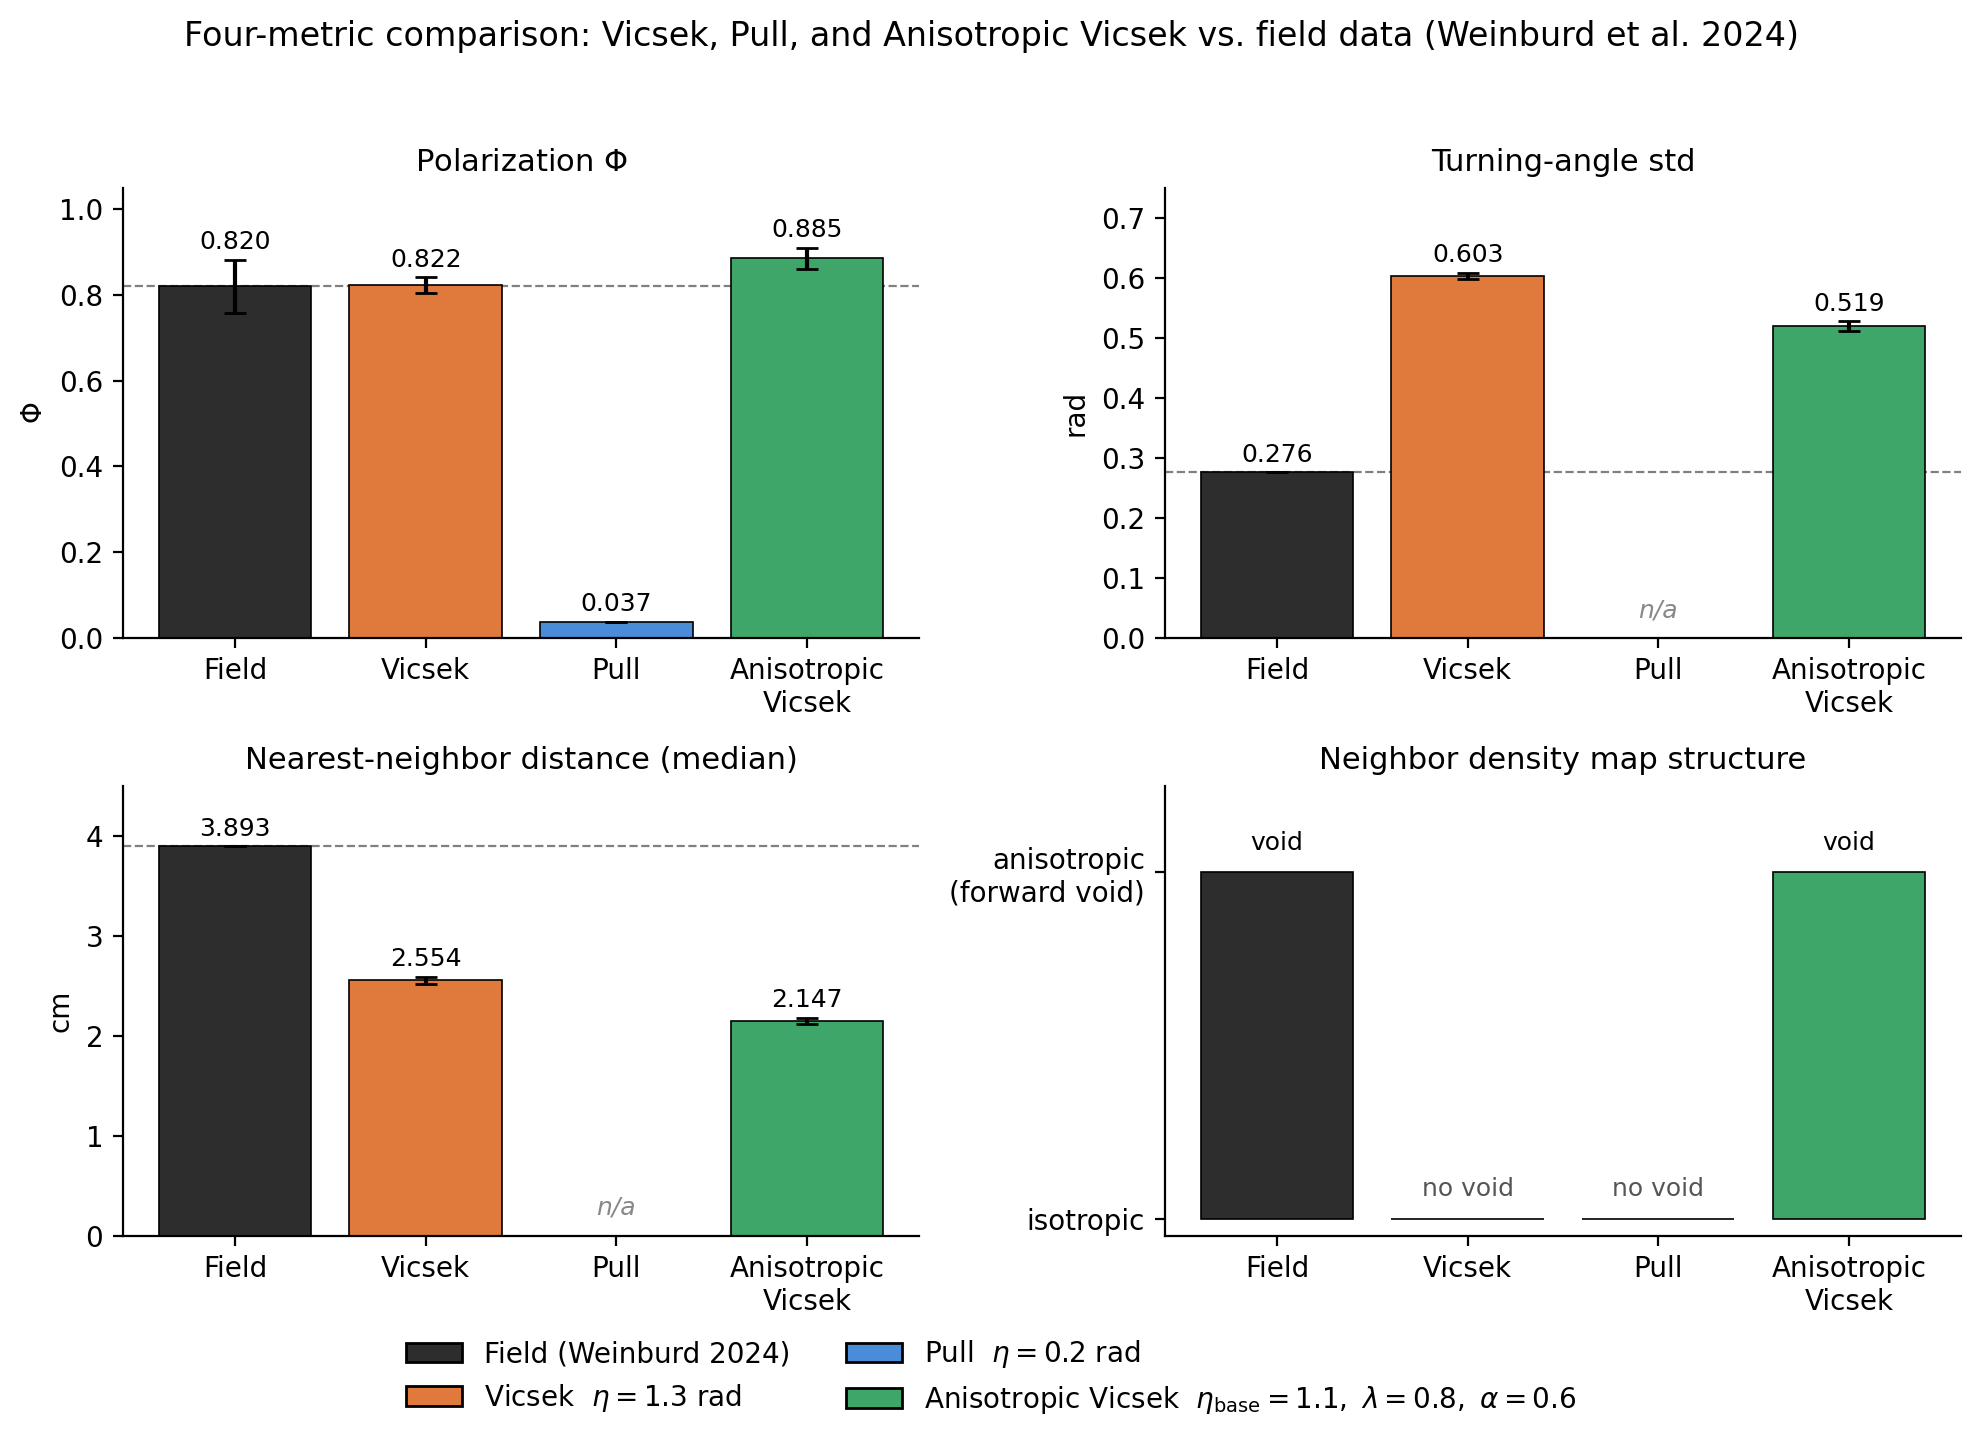
\includegraphics[width=\textwidth]{figures/figure1.png}
\caption{Four-metric comparison, all models vs.\ field data (Weinburd et al.\ 2024). Top row: polarization (mean $\pm$ std) and turning-angle standard deviation. Bottom row: NND median and neighbor density map structure (categorical: void present vs.\ absent). Vicsek matches polarization but produces turning-angle distributions $2.2\times$ wider than observed. Pull fails on polarization entirely. Anisotropic Vicsek matches polarization at reduced noise and is the only model to reproduce the forward void.}
\label{fig:summary}
\end{figure}

\subsection{Vicsek model}
Vicsek matches field polarization to within 0.2\% ($0.822 \pm 0.019$ vs.\ $0.820$) but requires $\eta = 1.3$ rad. At this noise level the model produces a turning-angle standard deviation $2.2\times$ larger than observed in the field ($0.603 \pm 0.005$ vs.\ $0.276$ rad), which we take as our primary measure of noise inflation. (We avoid directly comparing $\eta$ to the empirical turning-angle std because $\eta$ is a per-step angular noise injection sampled from $[-\eta/2, +\eta/2]$, while the empirical 0.276 rad is the observed frame-to-frame turning-angle std---the net result of whatever noise-plus-dynamics produces locust motion. The two quantities are related but not identical; the simulated turning-angle std is the appropriate comparison.) The NND median is 33\% below it (2.554 vs.\ 3.893 cm). The neighbor density map is isotropic at all tested parameter values.

Burn-in verification confirms steady-state equilibration across all 10 seeds well before the 20-second cutoff. Several seeds show brief direction-reversal events, consistent with finite-size effects in Vicsek-class models near the phase boundary.

The noise inflation has a direct mechanistic cause. Vicsek's alignment rule weights every neighbor equally regardless of position. In a swarm with no spatial structure to the interaction, the noise parameter must be large enough to allow the system to explore heading space and settle at the observed polarization, rather than being held at near-perfect polarization ($\Phi \to 1$) by strong isotropic consensus. The result is a noise level that predicts turning-angle distributions more than twice as wide as those measured in the field.

\subsection{Pull model: order destruction}
\label{sec:pull}
The pull model fails across all tested parameter combinations. Ensemble polarization is $0.037 \pm 0.001$, 4.5\% of the field target. A noise sweep from $\eta = 0.1$ to 2.9 rad gives a flat polarization response with no peak.

\begin{figure}[h]
\centering
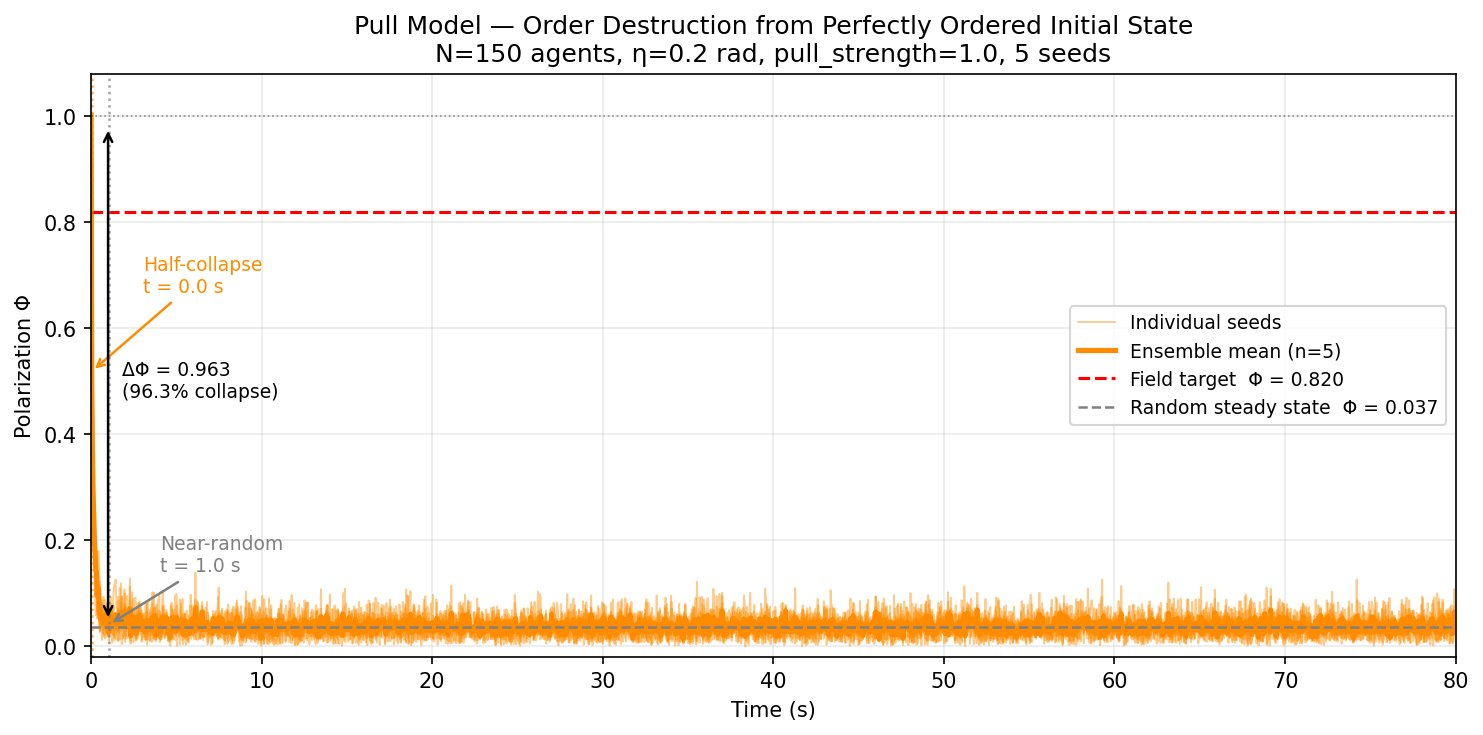
\includegraphics[width=0.9\textwidth]{figures/figure2.png}
\caption{Pull model initialized from near-perfect order ($\Phi = 1.000$) collapses to the disordered steady state ($\Phi \approx 0.037$) within 1 second across all 5 seeds. Half-collapse occurs within the first timestep ($dt = 0.04$ s). Steady-state polarization from ordered and random initialization are statistically identical ($0.037 \pm 0.001$ vs.\ $0.037 \pm 0.001$).}
\label{fig:pullcollapse}
\end{figure}

The ordered-initialization test rules out a bootstrapping explanation. Starting from $\Phi = 1.000$, the model collapses to the disordered steady state ($\Phi \approx 0.037$) within one second (Figure~\ref{fig:pullcollapse}). Half-collapse occurs in the first timestep ($dt = 0.04$ s), so the characteristic decay time is shorter than a single model update. Ordered and random initialization converge to identical steady states. The pull model does not merely fail to generate order: it actively destroys it.

The cause is geometric. When agents differ in heading by any amount, bearing angles toward neighbors are approximately uniformly distributed around each focal agent. The front-weighting function $w = \cos^2(\beta/2)$ down-weights rear neighbors but leaves front neighbors symmetric left-to-right, so their weighted circular mean provides no net lateral steering signal. More formally: any position-based steering rule whose weighting function is even under the $\beta \to -\beta$ reflection (as $\cos^2(\beta/2)$ is) produces, in expectation, zero lateral steering signal on an isotropic bearing distribution. Weak asymmetries introduced by small deviations from isotropy are washed out by heading noise before they can bias the distribution further. All five tested variants share this property.

This result is consistent with Sayin et al.'s emphasis on the ring-attractor circuit as a core component of the pull mechanism, though our simulations do not speak directly to the specific computational role of that circuit. What our results establish is narrower and, we think, sharper: no instantaneous, symmetric position-based rule of the class we tested can stabilize heading consensus on its own. Whatever additional machinery real locusts use (temporal integration, heading inertia, or an alternative we have not considered) it cannot be reduced to the per-timestep position-based steering rules of the kind typically included in SPP extensions.

\subsection{Anisotropic Vicsek: forward void emergence}
The Anisotropic Vicsek model (AV) is the only model to reproduce the forward void. Figure~\ref{fig:nd} shows the four-panel comparison: the field map has a pronounced anterior depletion, Vicsek and Pull are isotropic, and AV shows clear front-rear asymmetry.

\begin{figure}[h]
\centering
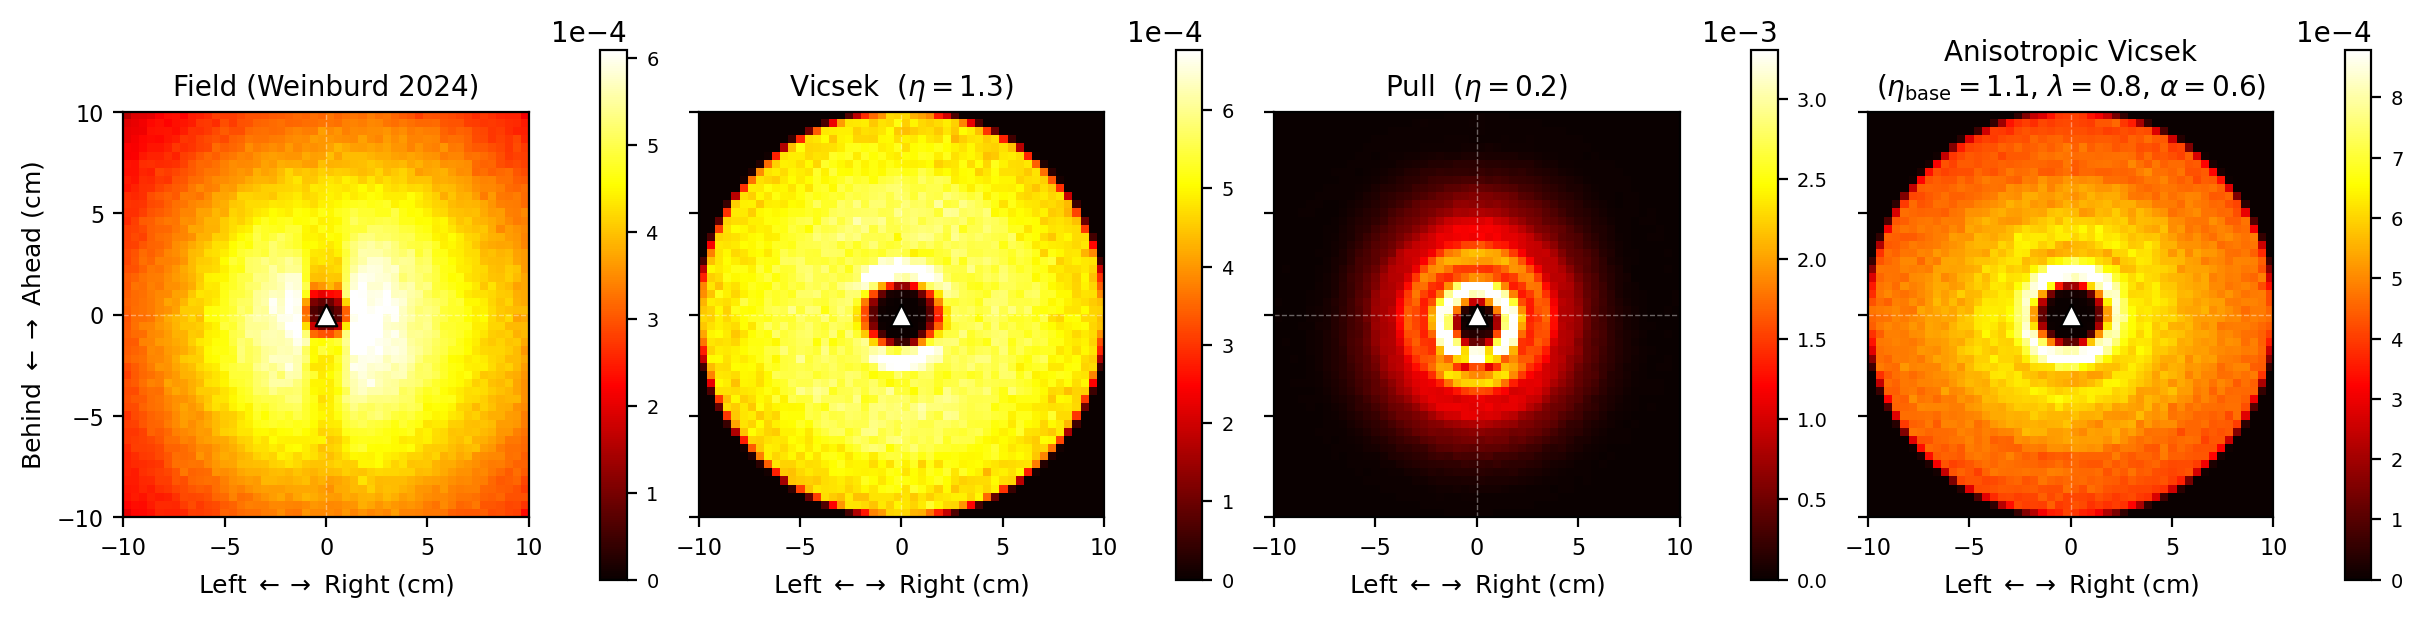
\includegraphics[width=\textwidth]{figures/figure3.png}
\caption{Body-centered neighbor density maps, focal heading up. Field data (far left) shows a forward void. Vicsek and Pull maps are isotropic. The Anisotropic Vicsek model (far right) reproduces the qualitative front-rear asymmetry. Colorbar: relative neighbor density.}
\label{fig:nd}
\end{figure}

AV over-predicts polarization by 7.9\% ($0.885 \pm 0.025$ vs.\ $0.820$) and under-predicts NND median by 44.8\% (2.147 vs.\ 3.893 cm). These are not independent failures. The forward-weighting that creates the void concentrates neighbors anteriorly and strengthens heading consensus, simultaneously driving up polarization and compressing inter-agent spacing. Increasing $\alpha$ to strengthen the void worsens both deviations; decreasing it reduces them but also eliminates the void. There is no $\alpha$ value at which all four metrics match.

\begin{figure}[h]
\centering
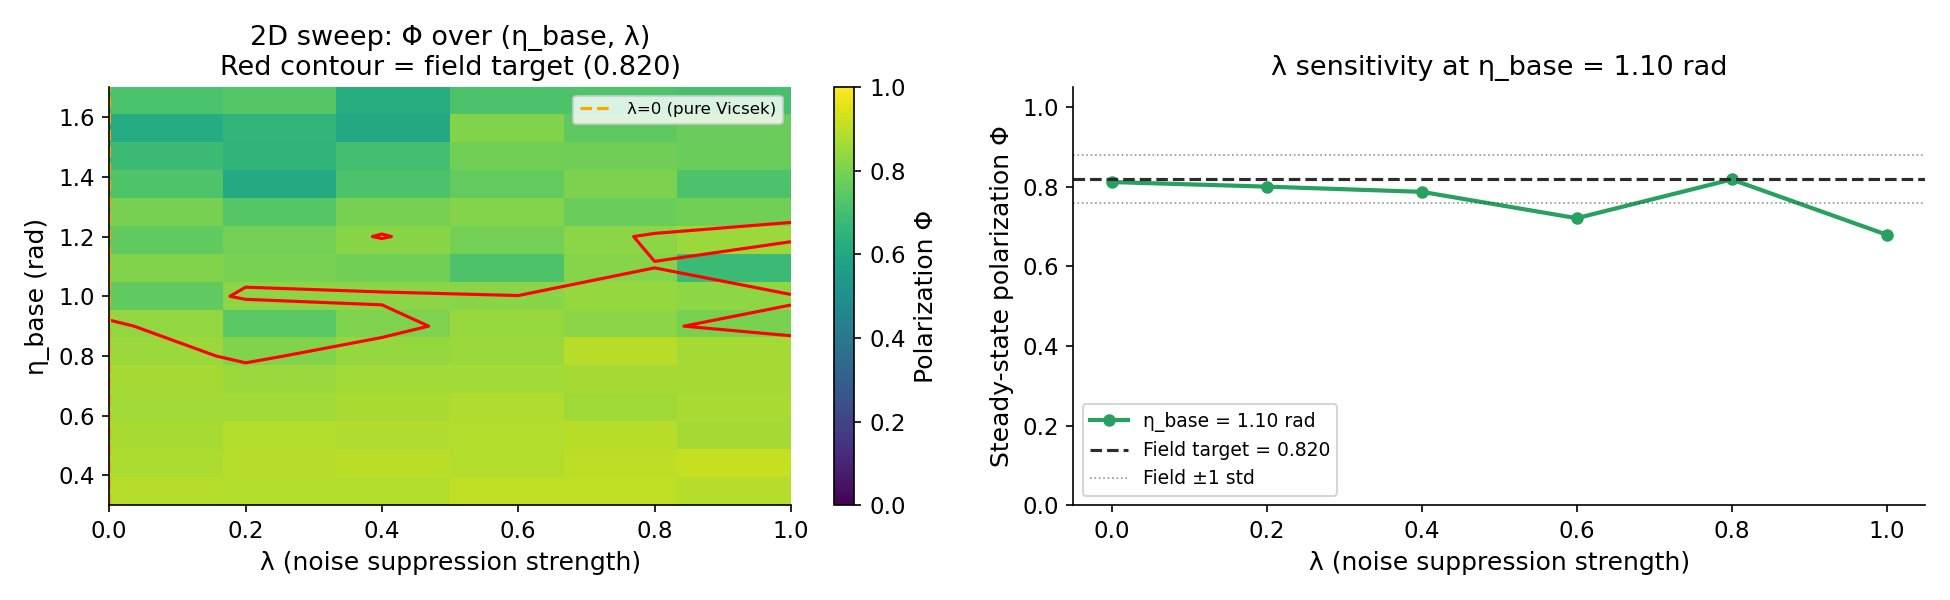
\includegraphics[width=\textwidth]{figures/figure4.png}
\caption{Left: 2D polarization sweep over ($\eta_{\mathrm{base}}, \lambda$). Red contour marks the field target (0.820). Right: $\lambda$ sensitivity at $\eta_{\mathrm{base}} = 1.1$ rad showing that polarization is stable across the $\lambda$ range. The $\alpha$ sweep (not shown) shows a monotonic tradeoff: at $\alpha = 0$ the density map is isotropic; at $\alpha = 1.0$ the void is strongest but polarization falls to 0.669.}
\label{fig:sweep}
\end{figure}

The $\lambda$ sweep confirms that noise suppression stabilizes but does not drive the polarization match: polarization holds near 0.82--0.89 across all tested $\lambda$ values at fixed $\eta_{\mathrm{base}}$. The void strength is controlled by $\alpha$, not $\lambda$. The operating point $\alpha = 0.6$ was chosen as the best achievable tradeoff between spatial anisotropy and scalar metric error.

\section{Discussion}

Three conclusions follow from these results. First, Vicsek provides a reasonable phenomenological fit to polarization but not to the spatial structure of real swarms. The $2.2\times$ inflation of simulated turning-angle std above the field value is not a calibration artifact: it reflects the model's inability to stabilize heading consensus through spatial asymmetry, forcing noise to do work it was not designed for. At the noise level required for polarization, the model predicts turning-angle distributions inconsistent with individual locust trajectories.

Second, an instantaneous position-based pull rule cannot produce collective alignment. The mechanism fails not because of missing parameter tuning but because the bearing distribution in any disordered swarm provides no net steering signal to an instantaneous rule. The ordered-initialization result strengthens this: the model does not merely fail to create order, it destroys existing order faster than any alignment mechanism can restore it. This is consistent with Sayin et al.'s emphasis on the ring-attractor circuit as central to the pull mechanism, but our simulations establish something narrower and more definite: whatever additional structure real locusts employ, it cannot be captured by the instantaneous, position-based rules that dominate SPP extensions. Temporal integration, heading inertia, or some combination is required.

Third, the forward void requires directional asymmetry in the interaction, but producing that asymmetry within an SPP framework generates over-alignment and over-clustering as coupled side effects. The AV model trades quantitative accuracy on two metrics to gain qualitative accuracy on the neighbor density map. This tradeoff appears to be a property of the model family rather than a parameter sensitivity: independent control of spatial structure and scalar statistics likely requires mechanisms not present in any of the three models, specifically heading inertia, attraction zones for spacing regulation, or temporal sensory integration.

Limitations worth noting: all simulations used periodic boundary conditions, while the field data were collected under open-boundary conditions. All three models under-predict NND by 33--45\%, and periodic boundaries are known to compress effective inter-agent distances; we cannot rule out that open boundaries would meaningfully narrow this gap. We flag this as the most important methodological caveat and a candidate for follow-up work. $N = 150$ agents is density-matched to the field arena but represents a small fraction of real band sizes; the AV parameter sweep was coarse and the selected parameters may not be jointly optimal; and the four metrics capture instantaneous spatial statistics only, omitting temporal autocorrelation and cluster-size distributions that could further distinguish the models.

\section{Conclusion}

None of the models we tested reproduces all four statistical signatures of real locust collective motion. Vicsek captures global order at the cost of spatial structure and requires noise levels inconsistent with individual trajectories. The pull model fails completely and, under both random and ordered initialization, actively destroys alignment, confirming that instantaneous position-based steering cannot substitute for temporal bearing integration. The Anisotropic Vicsek model recovers the forward void but cannot simultaneously match turning-angle and spacing statistics, revealing a tradeoff that is not resolvable by parameter adjustment alone. Closing the gap between SPP models and real locust motion will likely require heading inertia, explicit attraction zones, or a neural-level implementation of bearing integration.

\section*{References}
\begin{enumerate}\itemsep=0.2em
\item Buhl, J., Sumpter, D.\ J.\ T., Couzin, I.\ D., Hale, J.\ J., Despland, E., Miller, E.\ R., \& Simpson, S.\ J.\ (2006). From disorder to order in marching locusts. \emph{Science}, 312(5778), 1402--1406.
\item Couzin, I.\ D., Krause, J., James, R., Ruxton, G.\ D., \& Franks, N.\ R.\ (2002). Collective memory and spatial sorting in animal groups. \emph{Journal of Theoretical Biology}, 218(1), 1--11.
\item Krongauz, D.\ L., Ayali, A., \& Kaminka, G.\ A.\ (2024). Vision-based collective motion: A locust-inspired reductionist model. \emph{PLOS Computational Biology}, 20(1), e1011796.
\item Sayin, S., Couzin-Fuchs, E., Petelski, I., G\"unzel, Y., Salahshour, M., Lee, C.\ Y., Graving, J.\ M., Li, L., Deussen, O., Sword, G.\ A., \& Couzin, I.\ D.\ (2025). The behavioral mechanisms governing collective motion in swarming locusts. \emph{Science}, 387(6737), 995--1000.
\item Vicsek, T., Czir\'ok, A., Ben-Jacob, E., Cohen, I., \& Shochet, O.\ (1995). Novel type of phase transition in a system of self-driven particles. \emph{Physical Review Letters}, 75(6), 1226--1229.
\item Weinburd, J., Kasper, A., Dauphin, B., Garnier, S., \& Rundell, R.\ (2024). Anisotropic interaction and motion states of locusts in a hopper band [Dataset]. \emph{Dryad}. \url{https://doi.org/10.5061/dryad.n02v6wwzz}
\end{enumerate}

\section*{Project contributions}
Both authors contributed to experimental design, scientific interpretation, and writing throughout all phases of the project.

Asher Albrecht implemented the Vicsek model, built the Week 3 comparison notebook and Week 4 analysis notebook, and wrote all multi-seed validation and ordered-initialization scripts.

George Stephenson built the Week 1 data pipeline, implemented the Pull model and all five tested variants, and implemented the Anisotropic Vicsek model including the 2D parameter sweep.

Both authors jointly designed the Anisotropic Vicsek model specification, the analysis framework, and the scientific narrative. All code runs in a shared project directory on the Odysseus HPC cluster at CU Boulder.

\end{document}
